\newcommand{\Ps}{\mathcal P}

При помощи кода COSY Infinity мы вычисляем функцию спин-тюна $\nu_s(\vec z)$ в виде
разложения ряда Тэйлора, где
\begin{align*}
  \vec z &= (x,a,y,b,\ell,\delta), \\
  \ell &= -(t - t_0)v_0\frac{\gamma-1}{\gamma}, \\
  \delta &= \frac{\Delta K}{K}.
\end{align*}

В настоящем разделе, проверим утверждение 1 в обобщённой форме B: функцию многих переменных $\nu_s(\vec z)$
можно представить в виде функции скалярного параметра $\nu_s(\g*)$; при этом, мы не будем предполагать
никакого формального выражения параметра $\g*$.

Если формулировка B верна, то существует система координат (одной из осей которых является $\nu_s$),
в которой частицы, совершающие бетатронные колебания в горизонтальной плоскости, неотличимы,
с точки зрения спин-тюна, от частиц, совершающих колебания в вертикальной плоскости. К тому же, в этой системе координат не должны присутствовать координаты из поперечного
фазового пространства $(x,a)$, и $(y,b)$.

Таким образом, будем рассматривать пространство $\Ps=(\ell, \delta, \nu_s)$. Если формулировка B верна,
различие траекторий частиц в поперечном фазовом пространстве не должно отражаться на траектории частиц в $\Ps$.

В анализе использованы данные симуляции, описанной в предыдущем разделе.

На Рисунке~\ref{fig:main:all_ps} изображена зависимость $\nu_s(\vec z)$ от $(\ell, \delta)$ в том случае, когда
$\vec z$ представляет реальную фазовую координату частицы в ускорителе. Мы наблюдаем:
\begin{enumerate}
\item стратификацию среднего уровня спин-тюна, как мы это видели в симуляциях по подавлению декогеренции
  в разделе~\ref{sec:decoh:sim-imperfect};
  \item стратификация гораздо значительнее для X-банча (синие точки), чем для Y-банча (красные точки).
\end{enumerate}

Последнее объясняется большим значением функции дисперсии в горизонтальной плоскости. Отметим, что при одинаковом приведённом поперечном эмиттансе~\footnote{Приведённым эмиттансом будем называть произведение $\epsilon_\alpha\cdot Q_\alpha$, где $\alpha\in\{x,y\}$.} (то есть одинаковом удлинении орбит, если исходить из уравнения~\eqref{eq:betatron_OL}), частицы, совершающие бетатронные колебания в горизонтальной плоскости, обладают значительно большим продольным эмиттансом, чем совершающие колебания в вертикальной плоскости.

\begin{figure}[h]
  \centering
  \subbottom[Подобраны траектории с равными приведёнными поперечными эмиттансами.\label{fig:main:all_ps}]{%
    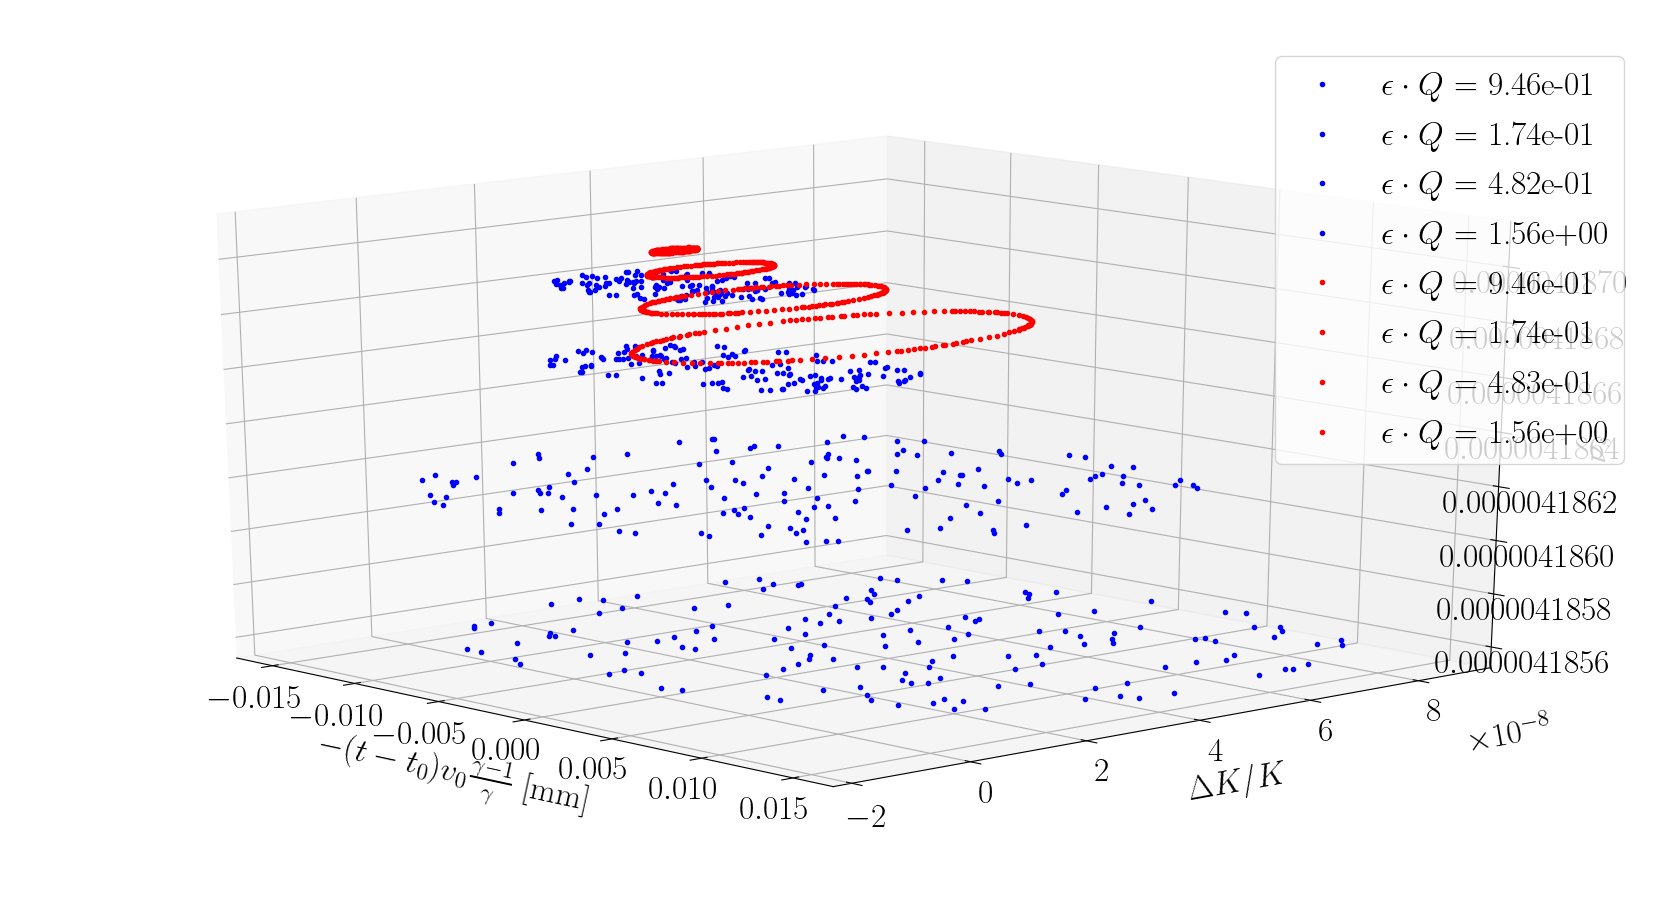
\includegraphics[height=.3\paperheight]{images/stune_traj_equ/part2/3D_plot_all_ps_vars}
    }
  \subbottom[Подобраны траектории с приблизительно равными продольными эмиттансами.\label{fig:main:gamma_eff}]{%
    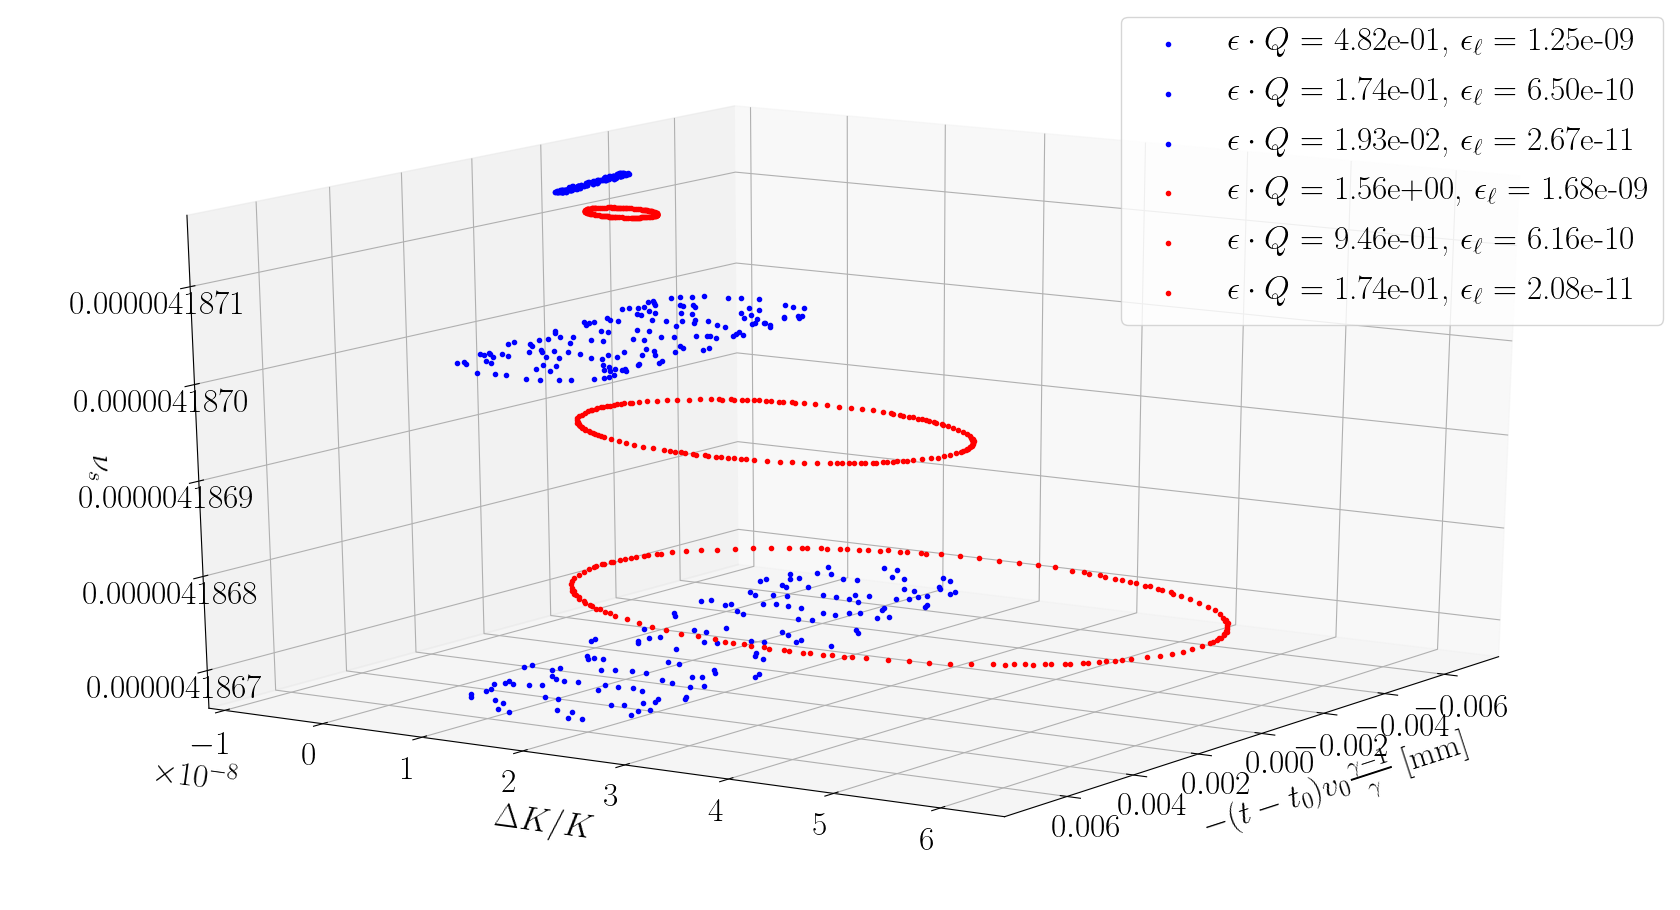
\includegraphics[height=.3\paperheight]{images/stune_traj_equ/part2/3D_plot_all_ps_vars_equal_long_emi}
    }
  \caption{Зависимость спин-тюна частицы от её положения в продольном фазовом пространстве.\label{fig:main}}
\end{figure}

В связи с последним, мы решили построить ту же самую зависимость, но подбирать пары частиц на основе равенства не приведённых поперечных эмиттансов, а на продольных эмиттансов. На Рисунке~\ref{fig:main:gamma_eff} мы наблюдаем, что частицы, с приблизительно одинаковыми продольными эмиттансами имеют приблизительно одинаковый уровень спин-тюна, независимо от плоскости совершения бетатронных колебаний.

\begin{figure}[h]
  \centering
  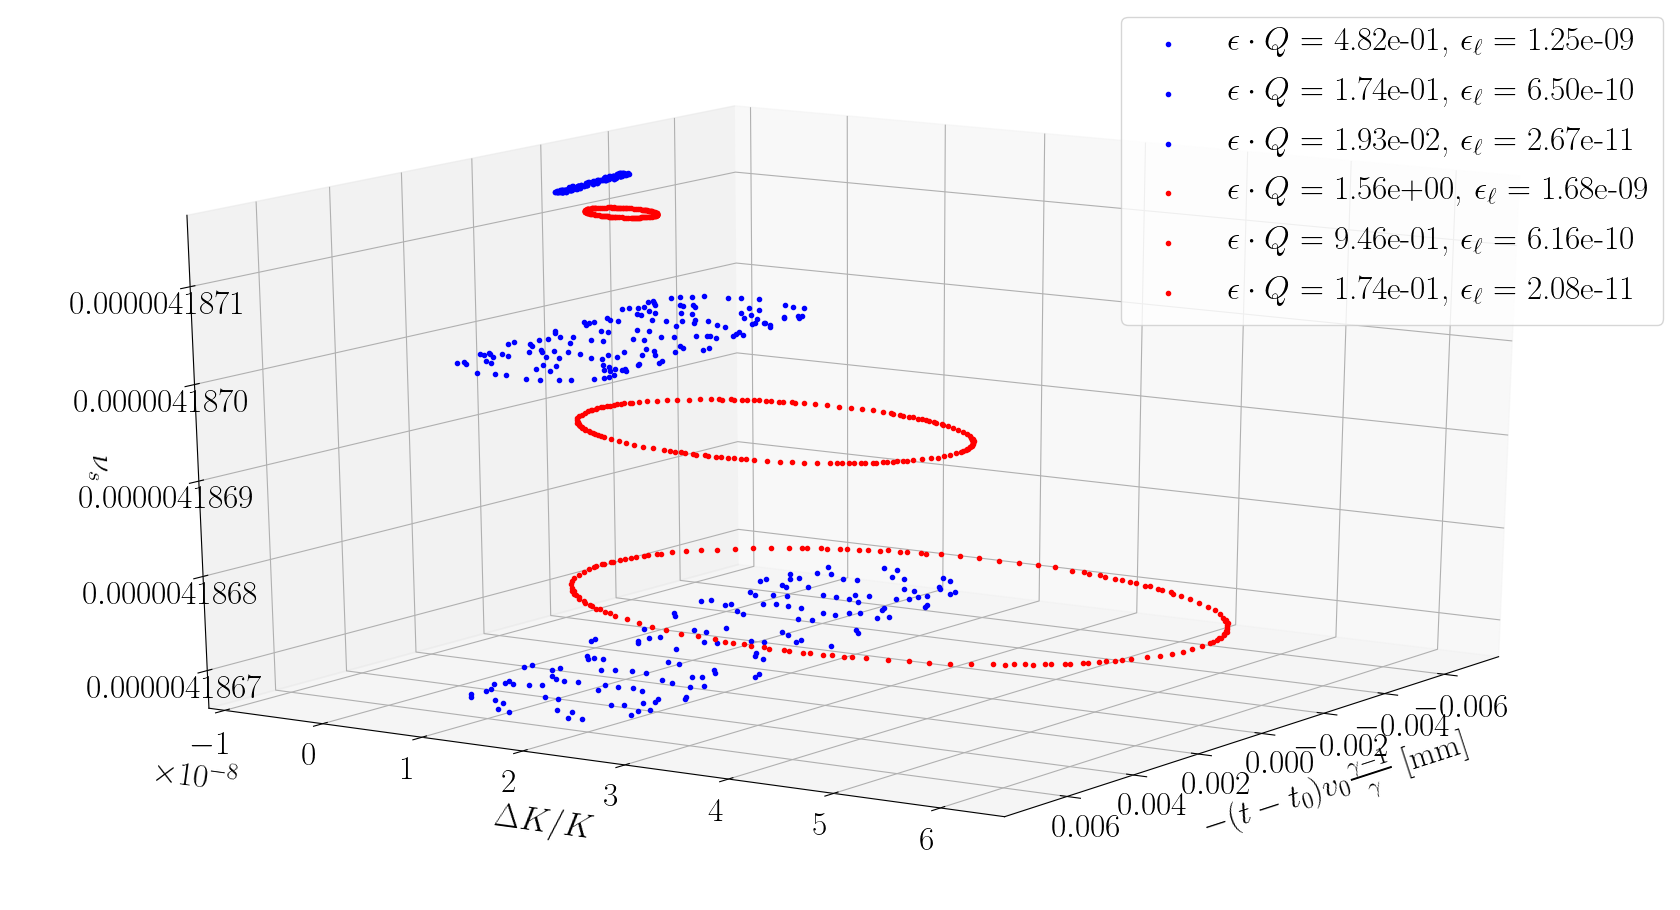
\includegraphics[height=.3\paperheight]{images/stune_traj_equ/part2/3D_plot_all_ps_vars_equal_long_emi}
  \caption{Подобраны траектории с приблизительно равными продольными эмиттансами.\label{fig:gamma_eff}}
\end{figure}

\paragraph{Вывод:} формулировка B подтверждается симуляцией; эффективный Лоренц-фактор отражает величину продольного эмиттанса частицы.
